% \documentclass[varwidth,10pt, border=10pt]{wlscirep}
\documentclass[varwidth, border=10pt, class=wlscirep, 10pt]{standalone}

\RequirePackage{helvet}
\RequirePackage{courier}

% border={10pt 5pt} % left/right bottom/top
% border={10pt 10pt 0pt 10pt} % left right bottom top


\usepackage{subcaption}
\usepackage[
    font=footnotesize,
    labelfont={bf,sf,footnotesize},
    labelsep=period,
    justification=raggedright
]{caption}
\usepackage{graphicx}

\begin{document}

\begin{figure}   % Figure 1
    \centering

    \begin{subfigure}[b]{6cm}
        \centering
        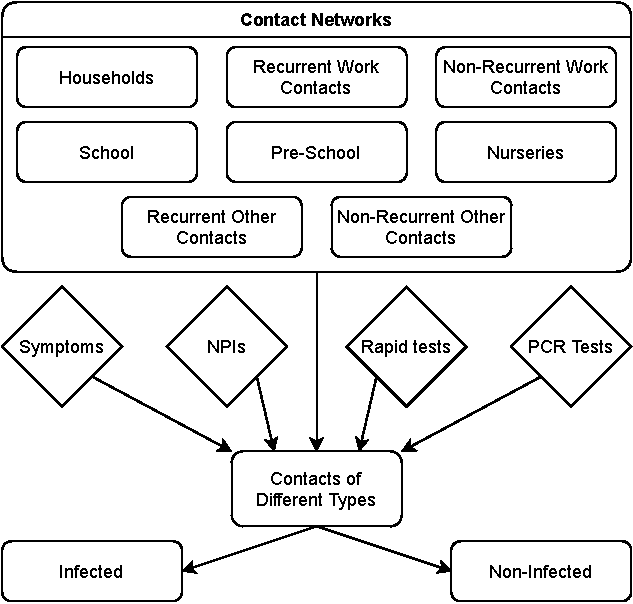
\includegraphics[width=5cm]{../figures/model-graph-top-left}
        \caption{Model for contacts and infections}
        \label{fig:model_contacts_infections}
    \end{subfigure}
    \hfill
    \begin{subfigure}[b]{6cm}
        \centering
        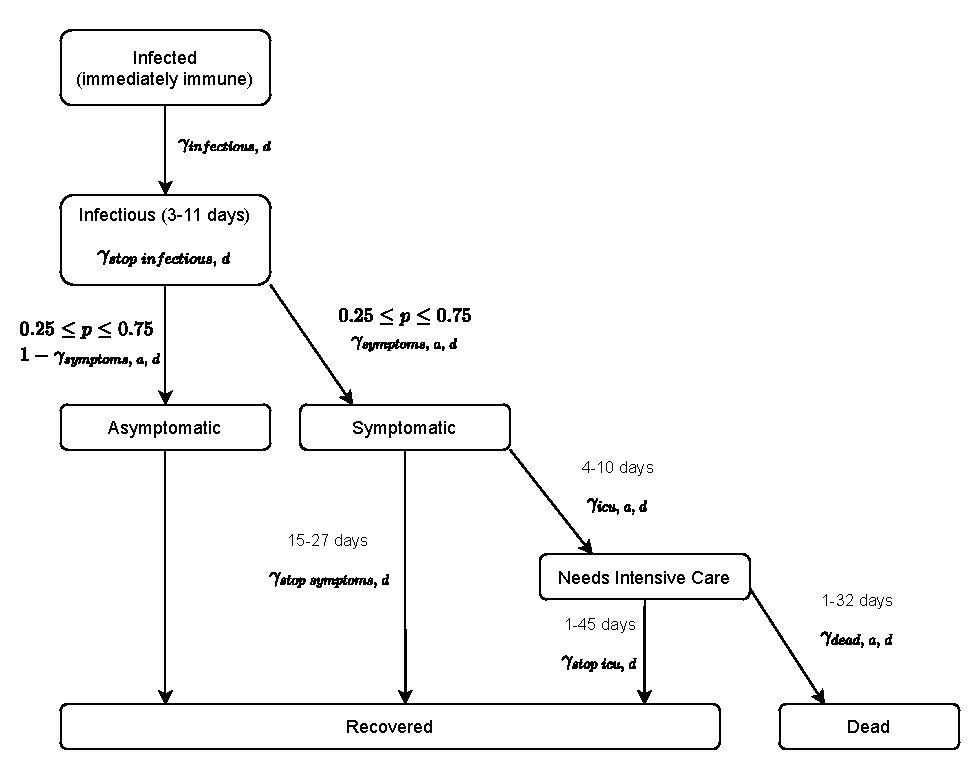
\includegraphics[width=5cm]{../figures/model-graph-top-right}

        \caption{Disease progression}
        \label{fig:model_disease_progression}
    \end{subfigure}
    \vskip3ex
    \begin{subfigure}[b]{6cm}
        \centering

        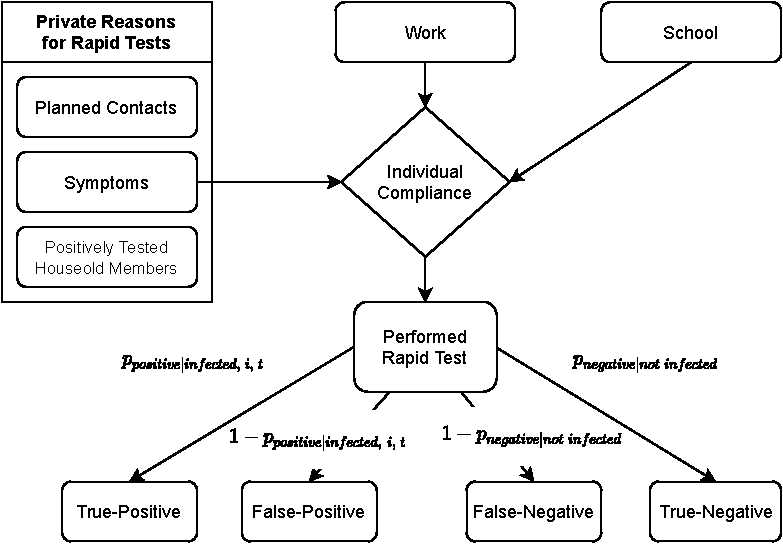
\includegraphics[width=5cm]{../figures/model-graph-bottom-left}
        \caption{Model for rapid tests}
        \label{fig:model_rapid_tests}
    \end{subfigure}
    \hfill
    \begin{subfigure}[b]{6cm}
        \centering
        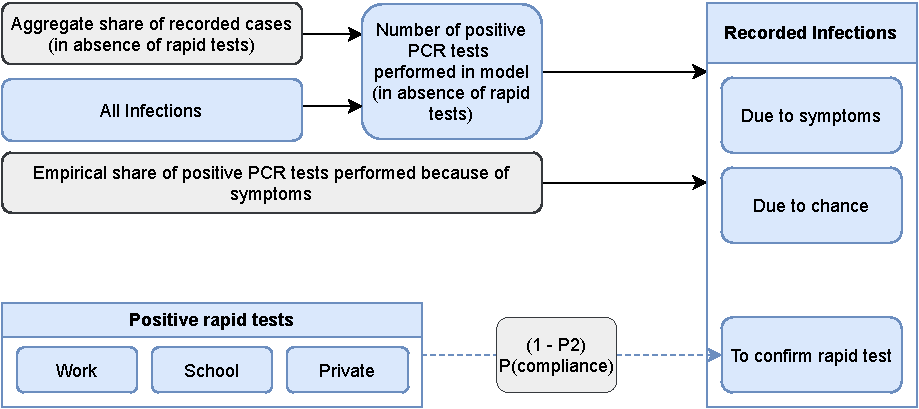
\includegraphics[width=5cm]{../figures/model-graph-bottom-right}

        \caption{Translating all infections to recorded ones}
        \label{fig:model_official_cases}
    \end{subfigure}

\end{figure}

\end{document}
